\chapter{Generative planning}

\begin{description}
    \item[Generative planning] \marginnote{Generative planning}
        Offline planning that creates the entire plan before execution based on
        a snapshot of the current state of the world.
        It relies on the following assumptions:
        \begin{descriptionlist}
            \item[Atomic time] 
                Actions cannot be interrupted.
            \item[Determinism] 
                Actions are deterministic.
            \item[Closed world] 
                The initial state is fully known, 
                what is not in the initial state is considered false (which is different from unknown).
            \item[No interference] Only the execution of the plan changes the state of the world.
        \end{descriptionlist}
\end{description}


\section{Linear planning}
\marginnote{Linear planning}
Formulates the planning problem as a search problem where:
\begin{itemize}
    \item Nodes contain the state of the world.
    \item Edges represent possible actions.
\end{itemize}
Produces a totally ordered list of actions.

The direction of the search can be:
\begin{descriptionlist}
    \item[Forward] \marginnote{Forward search}
        Starting from the initial state, the search terminates when a state containing a superset of the goal is reached.
    \item[Backward] \marginnote{Backward search}
        Starting from the goal, the search terminates when a state containing a subset of the initial state is reached.

        Goal regression is used to reduce the goal into sub-goals.
        Given a (sub-)goal $G$ and a rule (action) $R$ with delete-list (states that are false after the action) \texttt{d\_list}
        and add-list (states that are true after the action) \texttt{a\_list}, regression of $G$ through $R$ is define as:
        \[
            \begin{split}
                \texttt{regr[$G$, $R$]} &= \texttt{true} \text{ if } G \in \texttt{a\_list} \text{ (i.e. regression possible)} \\
                \texttt{regr[$G$, $R$]} &= \texttt{false} \text{ if } G \in \texttt{d\_list} \text{ (i.e. regression not possible)} \\
                \texttt{regr[$G$, $R$]} &= G \text{ otherwise} \text{ (i.e. $R$ does not influence $G$)} \\
            \end{split}  
        \]

        \begin{example}[Moving blocks]
            Given the action \texttt{unstack(X, Y)} with:
            \[
                \begin{split}
                    \texttt{d\_list} &= \{ \texttt{handempty}, \texttt{on(X, Y)}, \texttt{clear(X)} \} \\
                    \texttt{a\_list} &= \{ \texttt{holding(X)}, \texttt{clear(Y)} \}
                \end{split}
            \]
            We have that:
            \[
                \begin{split}
                    \texttt{regr[holding(b), unstack(b, Y)]} &= \texttt{true} \\
                    \texttt{regr[handempty, unstack(X, Y)]}  &= \texttt{false} \\
                    \texttt{regr[ontable(c), unstack(X, Y)]} &= \texttt{ontable(c)} \\
                    \texttt{regr[clear(c), unstack(X, Y)]} &= \begin{cases}
                        \texttt{true} & \text{if \texttt{Y}=\texttt{c}} \\
                        \texttt{clear(c)} & \text{otherwise}
                    \end{cases}
                \end{split}  
            \]
        \end{example}
\end{descriptionlist}


\subsection{Deductive planning}
\marginnote{Deductive planning}
Formulates the planning problem using first order logic to represent states, goals and actions.
Plans are generated as theorem proofs.

\subsubsection{Green's formulation}
\marginnote{Green's formulation}
Green's formulation is based on \textbf{situation calculus}.
To find a plan, the goal is negated and it is proven that it leads to an inconsistency.

The main concepts are:
\begin{descriptionlist}
    \item[Situation]
        Properties (fluents) that hold in a given state \texttt{s}.
        \begin{example}[Moving blocks]
            To denote that \texttt{ontable(c)} holds in a state \texttt{s}, we use the axiom:
            \[ \texttt{ontable(c, s)} \]
        \end{example}
        The operator \texttt{do} allows to evolve the state such that:
        \[ \texttt{do(A, S)} = \texttt{S'} \]
        \texttt{S'} is the new state obtained by applying the action \texttt{A} in the state \texttt{S}.

    \item[Actions]
        Define the pre-condition and post-condition fluents of an action in the form:
        \[ \texttt{pre-conditions} \rightarrow \texttt{post-conditions} \]
        Applying the equivalence $A \rightarrow B \equiv \lnot A \vee B$, actions can be described by means of disjunctions.
        \begin{example}[Moving blocks]
            The action \texttt{stack(X, Y)} has pre-conditions \texttt{holding(X)} and \texttt{clear(Y)}, and
            post-conditions \texttt{on(X, Y)}, \texttt{clear(X)} and \texttt{handfree}.
            Its representation in Green's formulation is:
            \[
                \begin{split}
                    \texttt{holding(X, S)} \land \texttt{clear(Y, S)} &\rightarrow \\
                    &\texttt{on(X, Y, do(stack(X, Y), s))} \land \\
                    &\texttt{clear(X, do(stack(X, Y), s))} \land \\
                    &\texttt{handfree(do(stack(X, Y), s))} \\
                \end{split}
            \]
        \end{example}

    \item[Frame axioms]
        Besides the effects of actions, each state also have to define for all non-changing fluents their frame axioms.
        If the problem is complex, the number of frame axioms becomes unreasonable.
        \begin{example}[Moving blocks]
            \[ \texttt{on(U, V, S)}, \texttt{diff(U, X)} \rightarrow \texttt{on(U, V, do(move(X, Y, Z), S))} \]
        \end{example}
\end{descriptionlist}


\begin{example}[Moving blocks]
    The initial state is described by the following axioms:\\[0.5em]
    \begin{minipage}{.3\linewidth}
        \centering
        \texttt{on(a, d, s0)} \\
        \texttt{on(b, e, s0)} \\
        \texttt{on(c, f, s0)} \\
        \texttt{clear(a, s0)} \\
        \texttt{clear(b, s0)} \\
    \end{minipage}
    \begin{minipage}{.3\linewidth}
        \centering
        \texttt{clear(c, s0)} \\
        \texttt{clear(g, s0)} \\
        \texttt{diff(a, b)} \\
        \texttt{diff(a, c)} \\
        \texttt{diff(a, d)} \dots \\
    \end{minipage}
    \begin{minipage}{.3\linewidth}
        \centering
        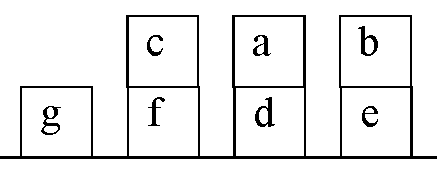
\includegraphics[width=\linewidth]{img/_moving_block_example_green.pdf}
    \end{minipage}\\[0.5em]

    For simplicity, we only consider the action \texttt{move(X, Y, Z)} that moves \texttt{X} from \texttt{Y} to \texttt{Z}.
    It is defined as:
    \[ 
        \begin{split}
            \texttt{clear(X, S)}&, \texttt{clear(Z, S)}, \texttt{on(X, Y, S)}, \texttt{diff(X, Z)} \rightarrow \\
            &\texttt{clear(Y, do(move(X, Y, Z), S))}, \texttt{on(X, Z, do(move(X, Y, Z), S))}
        \end{split}
    \]
    This action can be translated into the following effect axioms:
    \[ 
        \begin{split}
            \lnot\texttt{clear(X, S)} &\vee \lnot\texttt{clear(Z, S)} \vee \lnot\texttt{on(X, Y, S)} \vee \lnot\texttt{diff(X, Z)} \vee \\
            &\texttt{clear(Y, do(move(X, Y, Z), S))}
        \end{split}
    \]
    \[ 
        \begin{split}
            \lnot\texttt{clear(X, S)} &\vee \lnot\texttt{clear(Z, S)} \vee \lnot\texttt{on(X, Y, S)} \vee \lnot\texttt{diff(X, Z)} \vee \\
            &\texttt{on(X, Z, do(move(X, Y, Z), S))}
        \end{split}
    \]
\end{example}

Given the goal \texttt{on(a, b, s1)}, we prove that $\lnot\texttt{on(a, b, s1)}$ leads to an inconsistency.
We decide to make the following substitutions: 
\[ \{ \texttt{X}/\texttt{a}, \texttt{Z}/\texttt{b}, \texttt{s1}/\texttt{do(move(a, Y, b), S)} \} \]
The premise of \texttt{move} leads to an inconsistency (when applying \texttt{move} its premise is false):
\begin{center}
    \begin{tabular}{c|c|c|c}
        $\lnot\texttt{clear(a, S)}$ & $\lnot\texttt{clear(b, S)}$ & $\lnot\texttt{on(a, Y, S)}$ & $\lnot\texttt{diff(a, b)}$ \\
        False with $\{ \texttt{S}/\texttt{s0} \}$ & False with $\{ \texttt{S}/\texttt{s0} \}$ 
            & False with $\{ \texttt{S}/\texttt{s0}, \texttt{Y}/\texttt{d} \}$ & False
    \end{tabular}
\end{center}
Therefore, the substitution $\{ \texttt{s1}/\texttt{do(move(a, Y, b), S)} \}$ defines the plan to reach the goal \texttt{on(a, b, s1)}.


\subsubsection{Kowalsky's formulation}
\marginnote{Kowalsky's formulation}
Kowalsky's formulation avoids the frame axioms problem by using a set of fixed predicates:
\begin{descriptionlist}
    \item[\texttt{holds(rel, s/a)}] 
        Describes the relations \texttt{rel} that are true in a state \texttt{s} or after the execution of an action \texttt{a}.
    \item[\texttt{poss(s)}]
        Indicates if a state \texttt{s} is possible.
    \item[\texttt{pact(a, s)}]  
        Indicates if an action \texttt{a} can be executed in a state \texttt{s}.
\end{descriptionlist}
Actions can be described as:
\[ \texttt{poss(S)} \land \texttt{pact(A, S)} \rightarrow \texttt{poss(do(A, S))} \]

In the Kowalsky's formulation, each action requires a frame assertion (in Green's formulation, each state requires frame axioms).

\begin{example}[Moving blocks]
    An initial state can be described by the following axioms:\\[0.5em]
    \begin{minipage}{.35\linewidth}
        \centering
        \texttt{holds(on(a, b), s0)} \\
        \texttt{holds(ontable(b), s0)} \\
        \texttt{holds(ontable(c), s0)} \\
    \end{minipage}
    \begin{minipage}{.35\linewidth}
        \centering
        \texttt{holds(clear(a), s0)} \\
        \texttt{holds(clear(c), s0)} \\
        \texttt{holds(handempty, s0)} \\
        \texttt{poss(s0)} \\
    \end{minipage}
    \begin{minipage}{.2\linewidth}
        \centering
        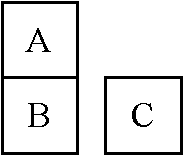
\includegraphics[width=0.6\linewidth]{img/_moving_block_example_kowalsky.pdf}
    \end{minipage}\\[0.5em]
\end{example}

\begin{example}[Moving blocks]
    The action \texttt{unstack(X, Y)} has:
    \begin{descriptionlist}
        \item[Pre-conditions] \texttt{on(X, Y)}, \texttt{clear(X)} and \texttt{handempty}
        \item[Effects] \phantom{}
        \begin{description}
            \item[Add-list] \texttt{holding(X)} and \texttt{clear(Y)}
            \item[Delete-list] \texttt{on(X, Y)}, \texttt{clear(X)} and \texttt{handempty}
        \end{description}
    \end{descriptionlist}

    Its description in Kowalsky's formulation is:
    \begin{descriptionlist}
        \item[Pre-conditions] 
            \[ 
                \begin{split}
                    \texttt{holds(on(X, Y), S)}&, \texttt{holds(clear(X), S)}, \texttt{holds(handempty, S)} \rightarrow \\
                    &\texttt{pact(unstack(X, Y), S)} 
                \end{split}
            \]
        
        \item[Effects] (use add-list)
            \[ \texttt{holds(holding(X), do(unstack(X, Y), S))} \]
            \[ \texttt{holds(clear(Y), do(unstack(X, Y), S))} \]
        
        \item[Frame condition] (uses delete-list)
            \[ 
                \begin{split}
                    \texttt{holds(V, S)}&, \texttt{V} \neq \texttt{on(X, Y)}, \texttt{V} \neq \texttt{clear(X)}, \texttt{V} \neq \texttt{handempty}
                    \rightarrow \\
                    & \texttt{holds(V, do(unstack(X, Y), S))}
                \end{split}
            \]
    \end{descriptionlist}
\end{example}


\subsection{STRIPS}
\marginnote{STRIPS}
STRIPS (Stanford Research Institute Problem Solver) is an ad-hoc algorithm
for linear planning resolution.
The elements of the problem are represented as:
\begin{descriptionlist}
    \item[State] represented with its true fluents.
    \item[Goal] represented with its true fluents.
    \item[Action] represented using three lists:
        \begin{descriptionlist}
            \item[Preconditions] Fluents that are required to be true in order to apply the action.
            \item[Delete-list] Fluents that become false after the action.
            \item[Add-list] Fluents that become true after the action.
        \end{descriptionlist}
        Add-list and delete-list can be combined in an effect list with positive (add-list) and negative (delete-list) axioms.

        \begin{description}
            \item[STRIPS assumption] Everything that is not in the add-list or delete-list is unchanged in the next state. 
        \end{description}
\end{descriptionlist}

STRIPS uses two data structures:
\begin{descriptionlist}
    \item[Goal stack] Does a backward search to reach the initial state.
    \item[Current state] Represents the forward application of the actions found using the goal stack.
\end{descriptionlist}

\begin{algorithm}
\caption{STRIPS}
\begin{lstlisting}[mathescape=true]
def strips(problem):
    goal_stack = Stack()
    current_state = State(problem.initial_state)
    goal_stack.push(problem.goal)
    plan = []
    while not goal_stack.empty():
        if (goal_stack.top() is a single/conjunction of goals and
            there is a substitution $\theta$ that makes it $\subseteq$ current_state):
            A = goal_stack.pop()
            $\theta$ = find_substitution(A, current_state)
            goal_stack.apply_substitution($\theta$)
        elif goal_stack.top() is a single goal:
            R = rule with a $\in$ R.add_list
            _ = goal_stack.pop() # Pop goal
            goal_stack.push(R)
            goal_stack.push(R.preconditions)
        elif goal_stack.top() is a conjunction of goals:
            for g in permutation(goal_stack.top()):
                goal_stack.push(g)
            # Note that there is no pop
        elif goal_stack.top() is an action:
            action = goal_stack.pop()
            current_state.apply(action)
            plan.append(action)
    return plan
\end{lstlisting}
\end{algorithm}

\begin{example}[Moving blocks] 
    \begin{center}
        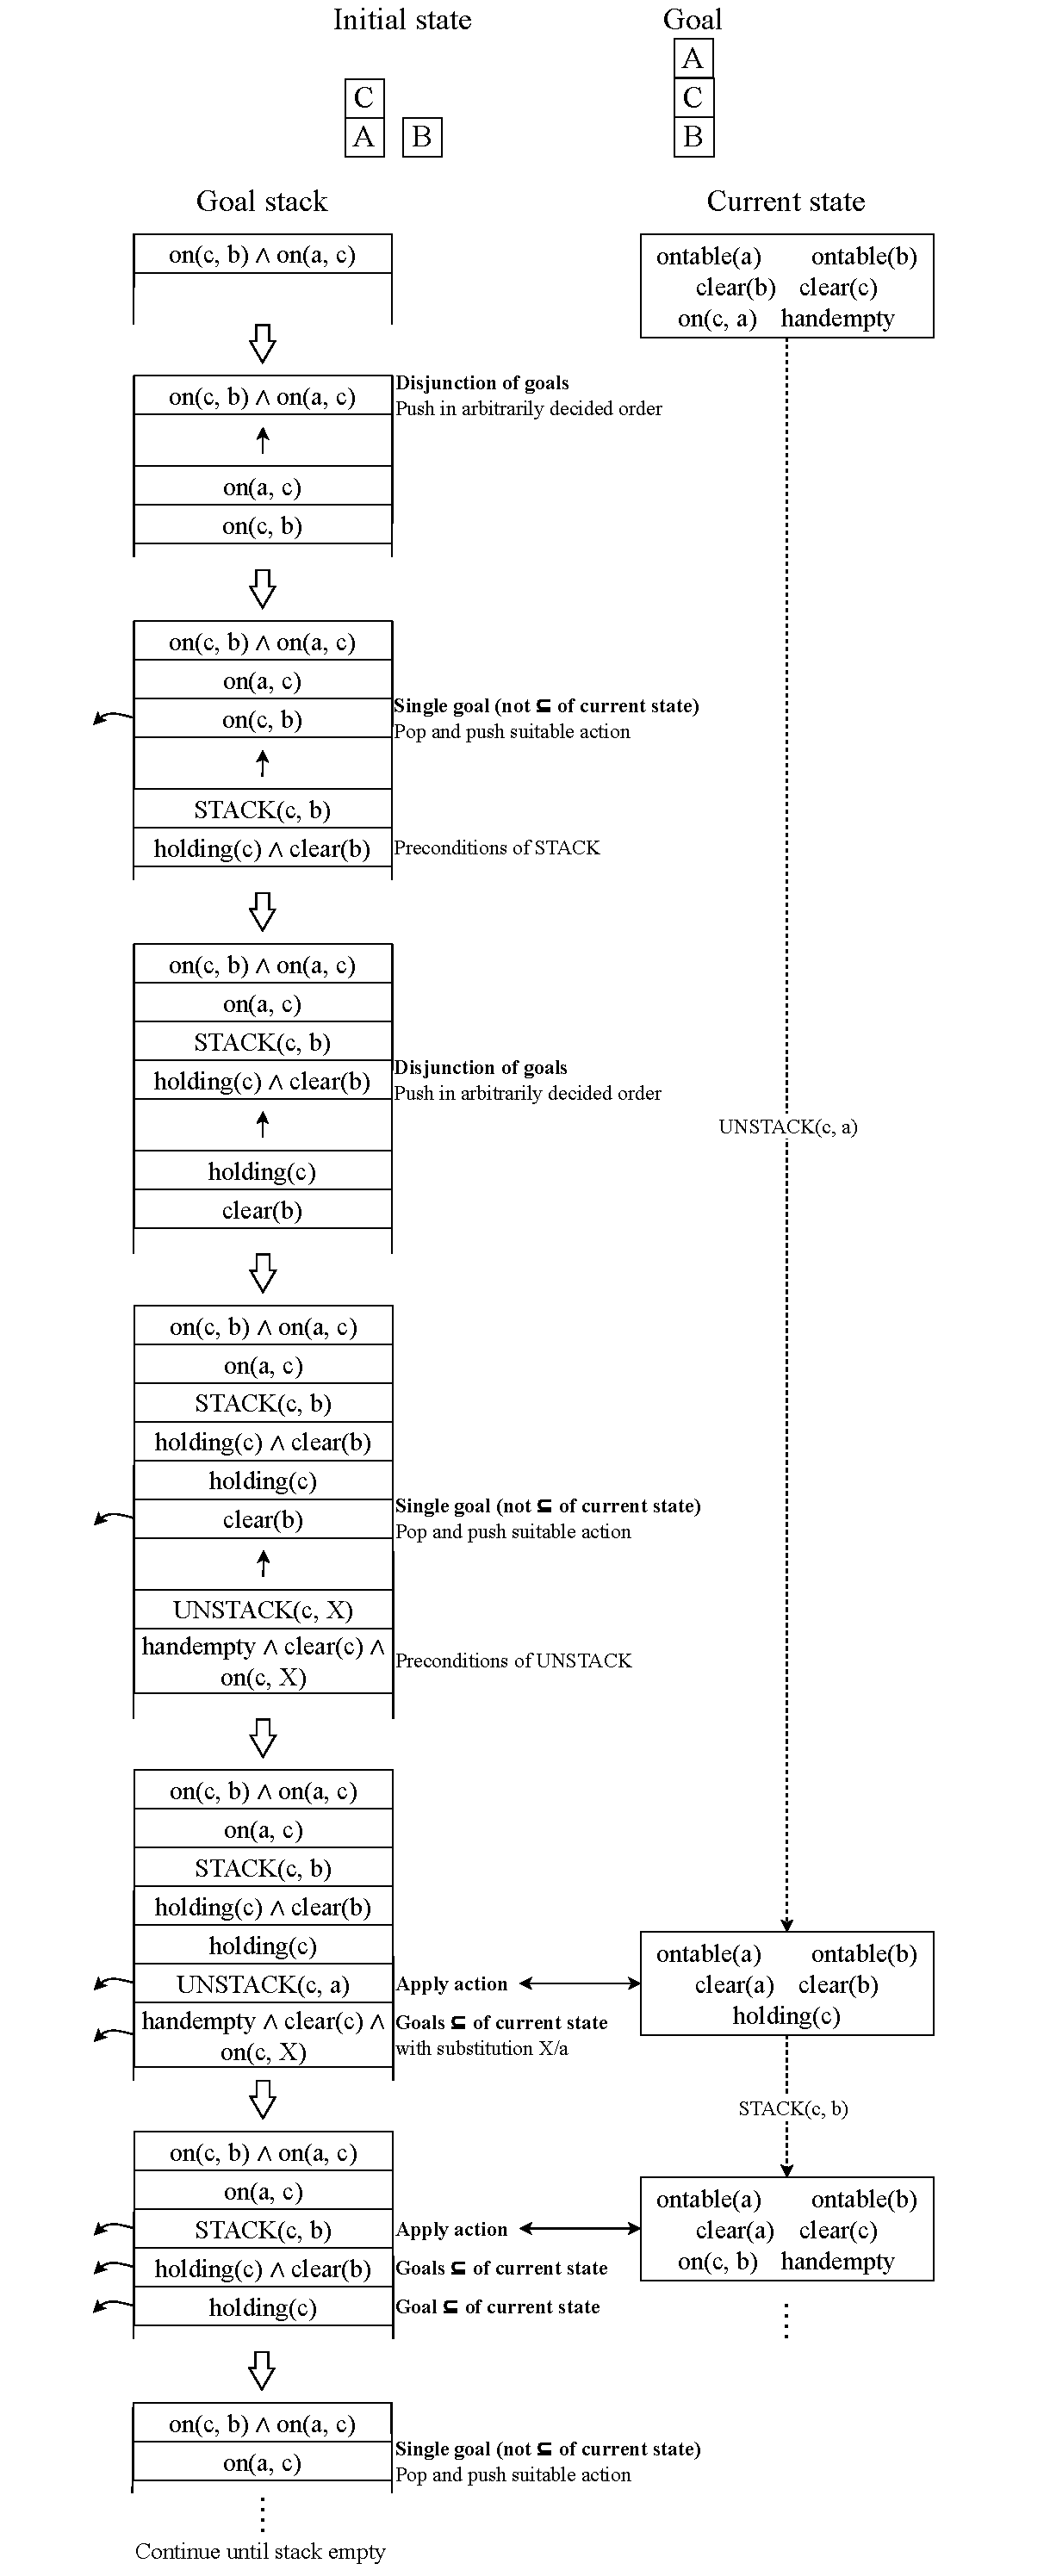
\includegraphics[trim={0 32.2cm 0 0}, clip, width=0.85\textwidth]{img/_strips_example.pdf}
    \end{center}
    \begin{center}
        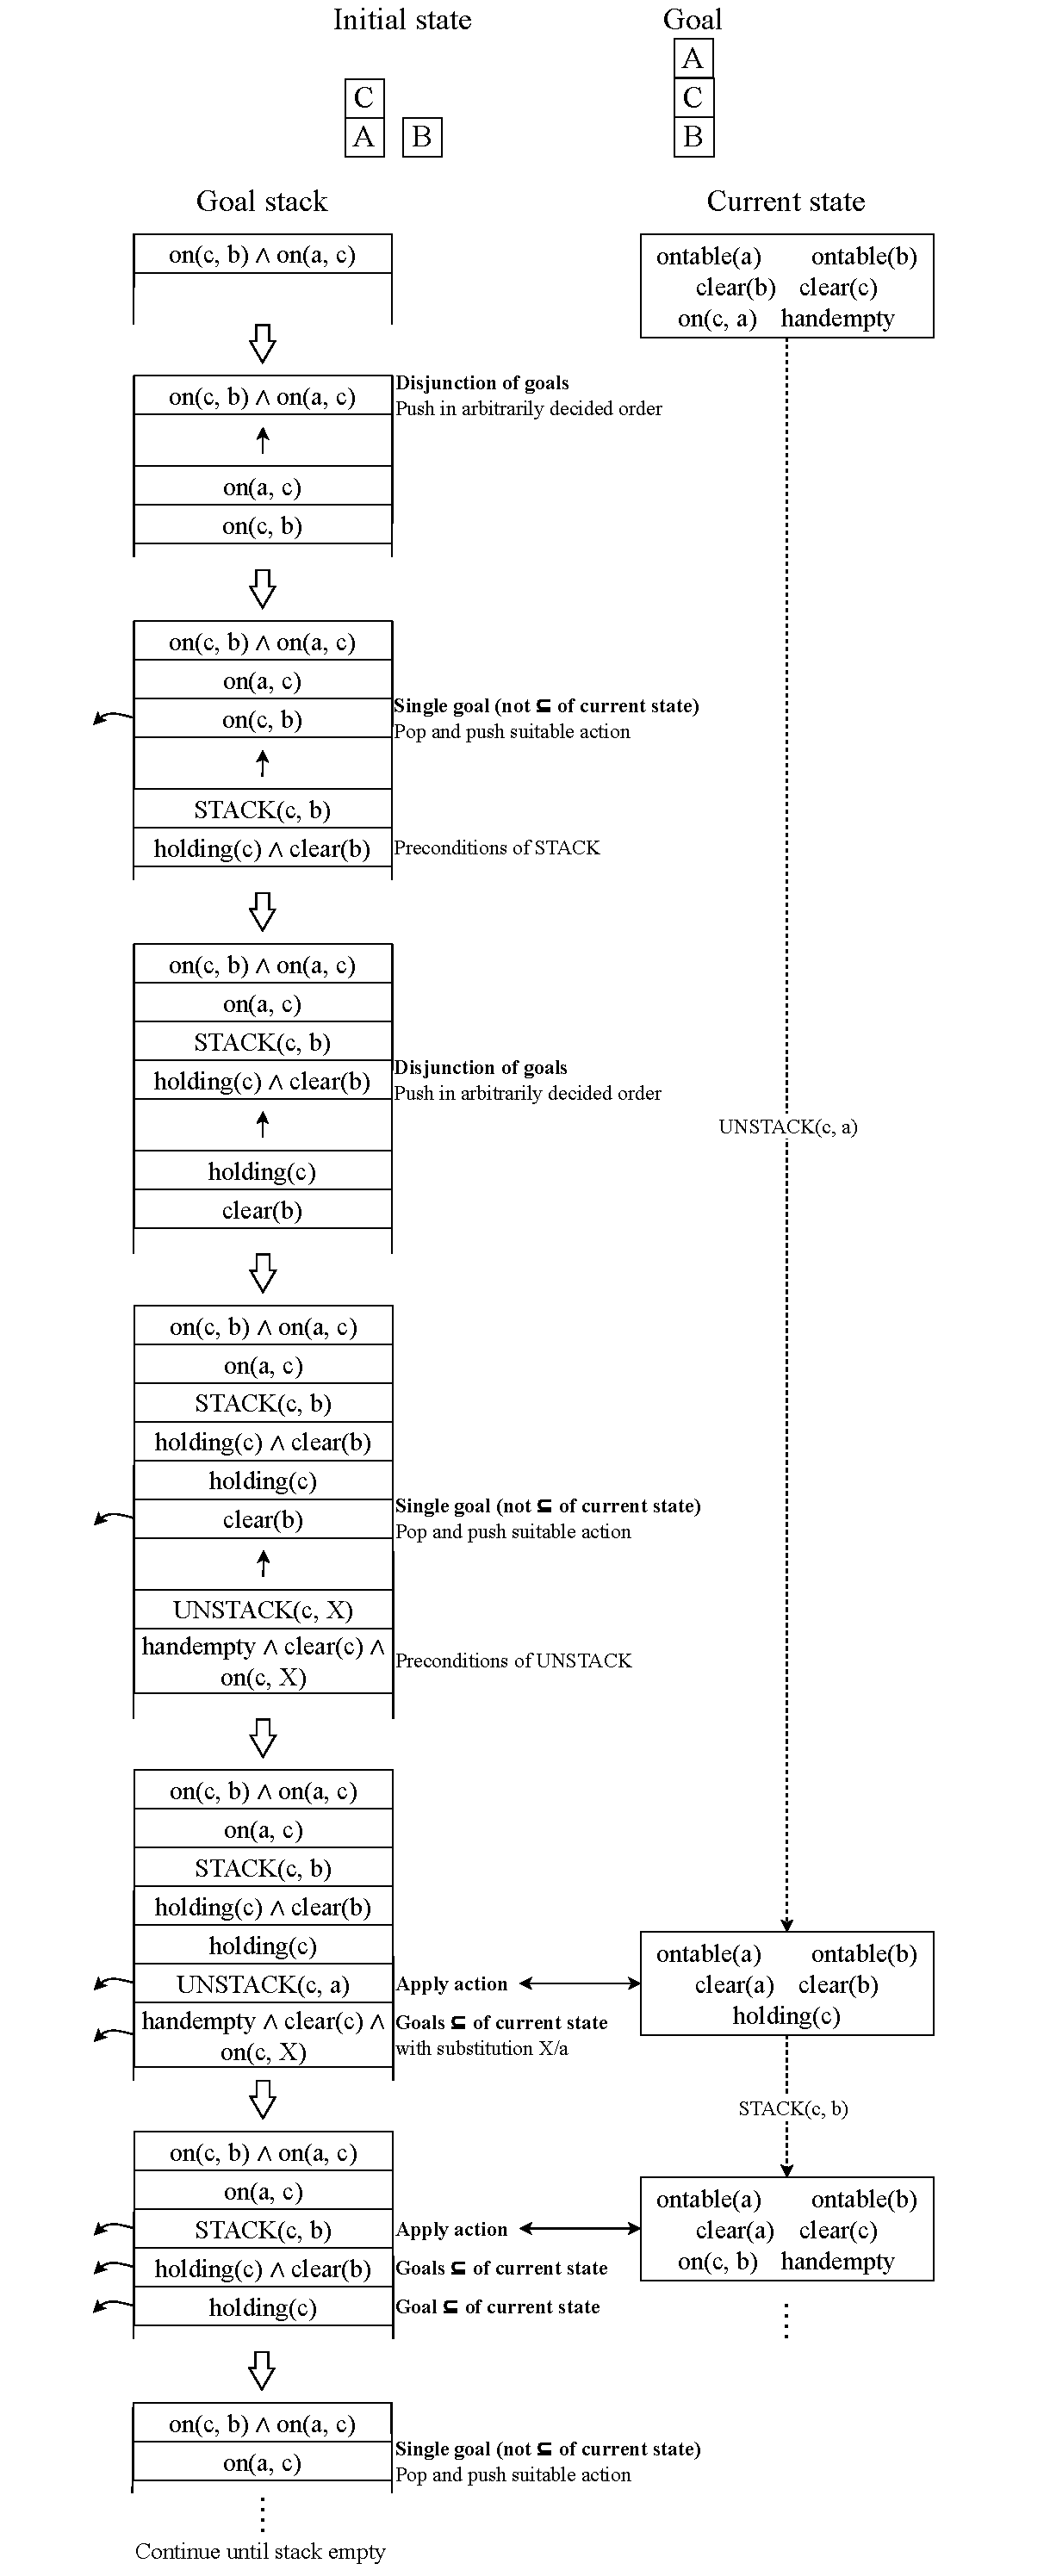
\includegraphics[trim={0 0 0 17.5cm}, clip, width=0.85\textwidth]{img/_strips_example.pdf}
    \end{center}
\end{example}

Since there are non-deterministic choices, the search space may become very large.
Heuristics may be used to avoid this.

Conjunction of goals are solved separately, but this could lead to the \marginnote{Sussman anomaly} \textbf{Sussman anomaly} 
where a sub-goal destroys what another sub-goal has done.
For this reason, when a conjunction is encountered, it is not immediately popped from the goal stack
and is left as a final check.